\documentclass[12pt]{article}
\usepackage[utf8]{inputenc}
\usepackage{amsmath}
\usepackage{amsfonts}
\usepackage{geometry}
\usepackage{titlesec}
\usepackage{tikz}
\geometry{a4paper, margin=1in}
\usetikzlibrary{positioning, calc, arrows.meta, shapes.geometric}


\title{Especificación Técnica: Modelo de Matriz de Conceptos Recursivos (ConceptMatrix 3D)}
\author{Arquitectura de Redes Neuronales Dispersas}
\date{Marzo 2026}

\begin{document}

\maketitle

\section{Introducción}
El modelo propuesto se define como una estructura de datos tridimensional dispersa, denotada como $CM$, donde cada coordenada activa $C(x, y, z)$ no solo representa un identificador semántico, sino que actúa como el punto de entrada a una red neuronal local $NN_c$.

\section{Estructura Espacial}
La matriz se define en un espacio euclidiano de tres dimensiones con una resolución $S$:
$$CM \in \mathbb{R}^{S \times S \times S}$$
Dada la naturaleza dispersa de la matriz, el conjunto de conceptos definidos $K$ es un subconjunto tal que $|K| \ll S^3$.

\section{El Nodo Conceptual como Red Neuronal}
Cada concepto $k \in K$ posee una función de transformación interna:
$$f_k(\mathbf{v}_{in}) = \sigma(W_k \cdot \mathbf{v}_{in} + b_k)$$
Donde:
\begin{itemize}
    \item $\mathbf{v}_{in}$ es el vector de contexto proveniente de conceptos adyacentes o de la entrada del sistema.
    \item $W_k$ es la matriz de pesos específica del concepto $k$, que representa miles de neuronas locales.
    \item $\sigma$ es la función de activación (ej. ReLU) que determina la relevancia del concepto en el flujo actual.
\end{itemize}

\section{Recursividad y Definición de Conceptos}
A diferencia de los modelos tradicionales, la salida de un nodo $C_i$ es una lista de punteros a otras coordenadas dentro de la misma matriz $CM$. La definición de un concepto "Carro" se expresa como:
$$\text{Def}(C_{carro}) = \{C_{motor}, C_{rueda}, C_{chasis}, \dots, C_n\}$$
Donde cada $C_i$ es, a su vez, una instancia de una red neuronal independiente.

\section{Proceso de Entrenamiento}
El entrenamiento del modelo se basa en la minimización de la distancia entre la trayectoria predicha por las redes neuronales y la trayectoria real definida en el corpus:

\subsection{Función de Pérdida (Loss Function)}
Para una secuencia de conceptos, la pérdida se calcula mediante la distancia euclidiana en el espacio 3D:
$$\mathcal{L} = \sum_{t=1}^{T} \| \hat{P}_t(x,y,z) - P_t(x,y,z) \|^2$$
Donde $\hat{P}_t$ es la coordenada predicha por la red del concepto actual y $P_t$ es la coordenada real del siguiente concepto en la definición.

\section{Conclusión}
Este modelo permite una navegación semántica basada en lógica estructural. La densidad de neuronas por cada punto de la matriz garantiza que el sistema no solo almacene posiciones, sino comportamientos dinámicos ante diferentes contextos lingüísticos.

\section{Arquitectura Interna del Nodo: Micro-Capas de Procesamiento}
Cada punto activo en la matriz $CM$ no es una unidad atómica, sino un contenedor de una arquitectura neuronal densa. Si definimos $N$ como el número de neuronas por concepto (donde $N \approx 1000$), el estado interno de un concepto se describe como un tensor de parámetros locales.

\subsection{Procesamiento de Contexto Local}
Cuando un concepto $C_k$ es activado, sus $N$ neuronas realizan una operación de filtrado selectivo sobre las señales de entrada $\mathbf{v}_{in}$. Esto permite que el concepto responda de manera distinta según el contexto:
$$ \mathbf{h}_k = \phi( \mathbf{W}_{local}^{(k)} \cdot \mathbf{v}_{in} + \mathbf{b}_{local}^{(k)} ) $$
Donde $\mathbf{h}_k \in \mathbb{R}^N$ representa el vector de estado oculto del concepto.

\subsection{Selección de Definición (Attention Mechanism)}
Dado que la definición de un concepto "Carro" contiene múltiples sub-conceptos $\{\text{motor, rueda, ...}\}$, las mil neuronas internas actúan como un mecanismo de atención que asigna pesos de relevancia $\alpha$ a cada hijo de la definición:
$$ \alpha_i = \text{softmax}( \text{score}(\mathbf{h}_k, C_i) ) $$
Esto permite que el modelo, ante la entrada "ruido en el motor", active con mayor intensidad la red neuronal del sub-concepto $C_{motor}$ que la del sub-concepto $C_{chasis}$.

\subsection{Aprendizaje de Micro-Pesos}
Durante la etapa de entrenamiento, el gradiente del error $\nabla \mathcal{L}$ se distribuye no solo para mover la posición $(x, y, z)$ del concepto en la matriz dispersa, sino para ajustar los miles de pesos internos $\mathbf{W}_{local}^{(k)}$. Esto permite que el concepto "aprenda" su propia semántica interna independientemente del resto de la matriz.

\section{Resolución de Limitaciones Intrínsecas de los LLMs Tradicionales}

La arquitectura de Matriz de Conceptos Recursiva (RCM) ofrece soluciones estructurales a los problemas de los modelos transformadores convencionales:

\subsection{Mitigación de Alucinaciones mediante Anclaje Semántico}
En los LLMs actuales, el conocimiento está distribuido de forma difusa. En este modelo, el conocimiento está \textit{localizado} en coordenadas $(x, y, z)$ y validado por su lista de sub-conceptos.
\begin{itemize}
    \item \textbf{LLM Tradicional:} Genera texto basado en la secuencia más probable, aunque sea falsa.
    \item \textbf{RCM:} Si la red neuronal del concepto "Carro" no tiene una conexión activa hacia el concepto "Volar", el modelo tiene una restricción física/lógica que le impide generar esa afirmación, eliminando la alucinación por diseño estructural.
\end{itemize}

\subsection{Razonamiento Simbólico-Neuronal (Neuro-Symbolic)}
Los LLMs tienen dificultades con la lógica multietapa. Al utilizar una estructura recursiva, este modelo realiza un "recorrido de grafo":
$$ \text{Pensamiento} = \text{Trayectoria}(C_{inicio} \to C_{def1} \to C_{sub-def} \dots) $$
Cada "salto" entre coordenadas requiere una activación de las mil neuronas locales, lo que obliga al modelo a mantener una coherencia lógica paso a paso, similar al razonamiento humano sistemático.

\subsection{Eficiencia Computacional y Actualización de Conocimiento}
Para enseñar un nuevo dato a un LLM actual, se debe re-entrenar todo el modelo (o gran parte de él). En la arquitectura RCM:
\begin{itemize}
    \item \textbf{Aprendizaje Localizado:} Si se descubre una nueva característica del "Motor", solo se actualizan los pesos $W_{local}^{(motor)}$ y su vector de coordenadas. El resto de la matriz permanece intacto.
    \item \textbf{Consumo de Recursos:} Solo se activan los conceptos relevantes para la consulta, en lugar de procesar billones de parámetros para cada palabra.
\end{itemize}


\section{Arquitectura Interna del Nodo: Micro-Capas de Procesamiento}
Cada punto activo en la matriz $CM$ no es una unidad atómica, sino un contenedor de una arquitectura neuronal densa. Si definimos $N$ como el número de neuronas por concepto (donde $N \approx 1000$), el estado interno de un concepto se describe como un tensor de parámetros locales.

\subsection{Procesamiento de Contexto Local}
Cuando un concepto $C_k$ es activado, sus $N$ neuronas realizan una operación de filtrado selectivo sobre las señales de entrada $\mathbf{v}_{in}$. Esto permite que el concepto responda de manera distinta según el contexto:
$$ \mathbf{h}_k = \phi( \mathbf{W}_{local}^{(k)} \cdot \mathbf{v}_{in} + \mathbf{b}_{local}^{(k)} ) $$
Donde $\mathbf{h}_k \in \mathbb{R}^N$ representa el vector de estado oculto del concepto.

\subsection{Selección de Definición (Attention Mechanism)}
Dado que la definición de un concepto "Carro" contiene múltiples sub-conceptos $\{\text{motor, rueda, ...}\}$, las mil neuronas internas actúan como un mecanismo de atención que asigna pesos de relevancia $\alpha$ a cada hijo de la definición:
$$ \alpha_i = \text{softmax}( \text{score}(\mathbf{h}_k, C_i) ) $$
Esto permite que el modelo, ante la entrada "ruido en el motor", active con mayor intensidad la red neuronal del sub-concepto $C_{motor}$ que la del sub-concepto $C_{chasis}$.

\subsection{Aprendizaje de Micro-Pesos}
Durante la etapa de entrenamiento, el gradiente del error $\nabla \mathcal{L}$ se distribuye no solo para mover la posición $(x, y, z)$ del concepto en la matriz dispersa, sino para ajustar los miles de pesos internos $\mathbf{W}_{local}^{(k)}$. Esto permite que el concepto "aprenda" su propia semántica interna independientemente del resto de la matriz.


\section{Resolución de Limitaciones Intrínsecas de los LLMs Tradicionales}

La arquitectura de Matriz de Conceptos Recursiva (RCM) ofrece soluciones estructurales a los problemas de los modelos transformadores convencionales:

\subsection{Mitigación de Alucinaciones mediante Anclaje Semántico}
En los LLMs actuales, el conocimiento está distribuido de forma difusa. En este modelo, el conocimiento está \textit{localizado} en coordenadas $(x, y, z)$ y validado por su lista de sub-conceptos.
\begin{itemize}
    \item \textbf{LLM Tradicional:} Genera texto basado en la secuencia más probable, aunque sea falsa.
    \item \textbf{RCM:} Si la red neuronal del concepto "Carro" no tiene una conexión activa hacia el concepto "Volar", el modelo tiene una restricción física/lógica que le impide generar esa afirmación, eliminando la alucinación por diseño estructural.
\end{itemize}

\subsection{Razonamiento Simbólico-Neuronal (Neuro-Symbolic)}
Los LLMs tienen dificultades con la lógica multietapa. Al utilizar una estructura recursiva, este modelo realiza un "recorrido de grafo":
$$ \text{Pensamiento} = \text{Trayectoria}(C_{inicio} \to C_{def1} \to C_{sub-def} \dots) $$
Cada "salto" entre coordenadas requiere una activación de las mil neuronas locales, lo que obliga al modelo a mantener una coherencia lógica paso a paso, similar al razonamiento humano sistemático.

\subsection{Eficiencia Computacional y Actualización de Conocimiento}
Para enseñar un nuevo dato a un LLM actual, se debe re-entrenar todo el modelo (o gran parte de él). En la arquitectura RCM:
\begin{itemize}
    \item \textbf{Aprendizaje Localizado:} Si se descubre una nueva característica del "Motor", solo se actualizan los pesos $W_{local}^{(motor)}$ y su vector de coordenadas. El resto de la matriz permanece intacto.
    \item \textbf{Consumo de Recursos:} Solo se activan los conceptos relevantes para la consulta, en lugar de procesar billones de parámetros para cada palabra.
\end{itemize}

\section{Mecanismo de Comunicación: Paso de Mensajes Dinámico}
La interacción entre nodos conceptuales $C_i$ y $C_j$ se define mediante una función de transferencia de mensajes $M$:
$$ \mathbf{m}_{i \to j} = \text{MLP}_{local}^{(i)}(\mathbf{h}_i) $$
Donde el mensaje $\mathbf{m}$ es un vector proyectado desde el estado oculto del concepto emisor. El concepto receptor actualiza su estado mediante:
$$ \mathbf{h}_j^{(t+1)} = \text{Update}(\mathbf{h}_j^{(t)}, \sum_{i \in \text{Def}(C_j)} \mathbf{m}_{i \to j}) $$
Este proceso permite que la matriz disperse información de manera asíncrona y dirigida, evitando la saturación del espacio de cómputo.




\begin{figure}[h]
	\centering
	% Ajustamos el tamaño general del lienzo
	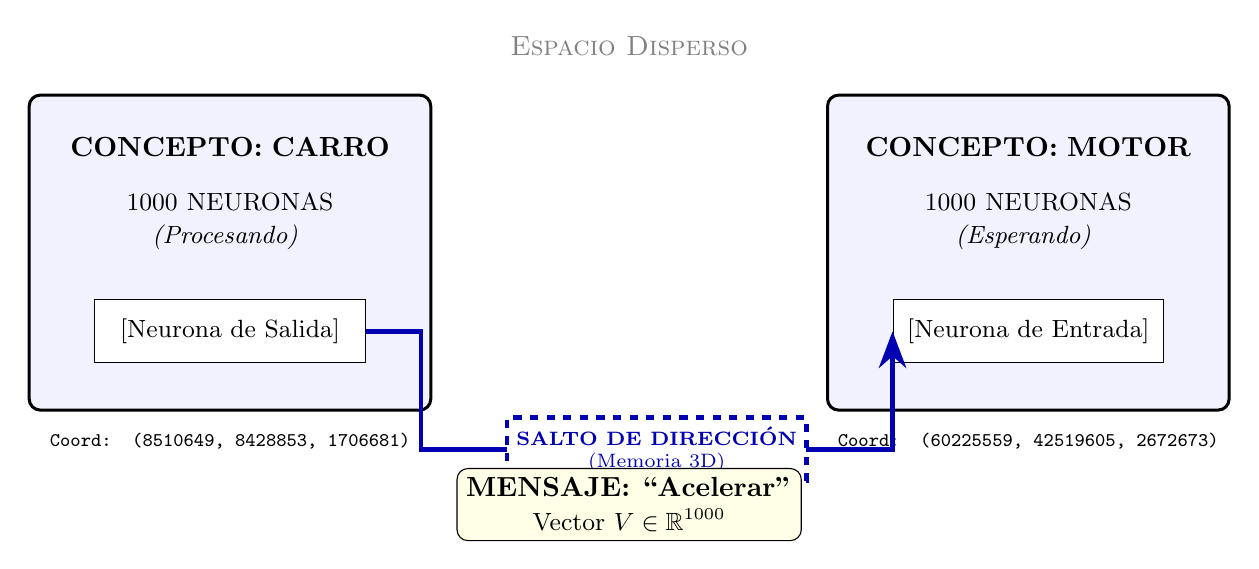
\begin{tikzpicture}[
		node distance=2cm and 2.5cm,
		% --- ESTILO CORREGIDO PARA DAR ESPACIO ---
		concept/.style={
			rectangle, 
			draw, 
			fill=blue!5, 
			% Aumentamos el ancho del texto a 4.5cm
			text width=4.5cm, 
			% Aumentamos la altura mínima a 4.0cm
			minimum height=4.0cm, 
			% Añadimos un margen interno de 0.3cm
			inner sep=0.3cm,
			rounded corners, 
			line width=1.1pt, 
			align=center
		},
		neuron_box/.style={
			rectangle, 
			draw, 
			fill=white, 
			text width=3.2cm, 
			minimum height=0.8cm, 
			align=center, 
			font=\small
		},
		msg_arrow/.style={
			-{Stealth[scale=1.3]}, 
			line width=1.6pt, 
			color=blue!70!black
		}
		]
		
		% --- CONCEPTO: CARRO ---
		\node (carro) [concept] {
			\textbf{CONCEPTO: CARRO}\\
			\vspace{0.3cm}
			\small 1000 NEURONAS\\
			\textit{(Procesando)}
			\vspace{1.5cm} % Espacio extra para la neurona de salida
		};
		\node [below=0.15cm of carro, font=\ttfamily\scriptsize] {Coord: (8510649, 8428853, 1706681)};
		
		% Neurona de salida colocada manualmente dentro del cuadro
		\node (out) [neuron_box, shift={(0,-1.0)}] at (carro.center) {[Neurona de Salida]};
		
		% --- CONCEPTO: MOTOR ---
		% Aumentamos la distancia relativa a 5cm
		\node (motor) [concept, right=5cm of carro] {
			\textbf{CONCEPTO: MOTOR}\\
			\vspace{0.3cm}
			\small 1000 NEURONAS\\
			\textit{(Esperando)}
			\vspace{1.5cm} % Espacio extra para la neurona de entrada
		};
		\node [below=0.15cm of motor, font=\ttfamily\scriptsize] {Coord: (60225559, 42519605, 2672673)};
		
		% Neurona de entrada colocada manualmente dentro del cuadro
		\node (in) [neuron_box, shift={(0,-1.0)}] at (motor.center) {[Neurona de Entrada]};
		
		% --- ESPACIO DISPERSO ---
		\node at ($(carro.north)!0.5!(motor.north) + (0,0.6)$) [font=\scshape\color{gray}] {Espacio Disperso};
		
		% --- CONEXIÓN Y SALTO ---
		% Dibujamos la línea que sale, baja y entra
		\draw [msg_arrow] (out.east) -- ++(0.7,0) -- ++(0,-1.5) -| node[pos=0.25, fill=white, draw, dashed, font=\scriptsize, align=center] {
			\textbf{SALTO DE DIRECCIÓN}\\
			(Memoria 3D)
		} (in.west);
		
		% --- ETIQUETA DEL MENSAJE ---
		% Colocamos el mensaje más abajo para que no choque con la línea
		\node at ($(carro)!0.5!(motor) + (0,-3.2)$) [align=center, draw, fill=yellow!10, rounded corners] {
			\textbf{MENSAJE: ``Acelerar''}\\
			\small Vector $V \in \mathbb{R}^{1000}$
		};
		
	\end{tikzpicture}
	\caption{Arquitectura de comunicación punto a punto en ConceptMatrix.}
\end{figure}


\section{Operativa del Modelo ConceptMatrix}

\begin{itemize}
    \item \textbf{Propiedades del Diseño Estructural:}
    \begin{description}
        \item[Desacoplamiento:] La red de "Carro" no posee una conexión física persistente con la de "Motor". La comunicación se establece mediante la resolución de la "dirección postal" (coordenada 3D) almacenada en los punteros de definición, permitiendo una topología modular.
        \item[Carga Dinámica:] Optimización de recursos mediante la activación selectiva. Solo se instancian en memoria RAM las micro-redes de los conceptos involucrados en el flujo de mensajes activo, manteniendo el resto de la matriz dispersa en un estado de reposo computacional.
    \end{description}

    \item \textbf{Mecanismos de Comunicación Inter-Conceptual:}
\end{itemize}

\begin{enumerate}
    \item \textbf{Bus de Mensajes Global (Vector de Contexto):} 
    Funciona como un espacio de trabajo compartido de corto plazo. Cuando el nodo "Carro" se activa, genera un \textit{Vector de Mensaje} (ej. semántica de "velocidad"). El sistema direcciona este vector hacia las 1000 neuronas del nodo "Motor", las cuales lo procesan como un \textit{input} adicional para modular su respuesta específica al contexto.
    
    \item \textbf{Direccionamiento por Punteros (Pointer Networks):} 
    Las neuronas especializadas dentro de cada concepto actúan como emisores de direcciones. El nodo "Carro" emite el valor exacto de la coordenada de destino $(60225559, 42519605, 2672673)$. Este "hipervínculo neuronal" permite saltos eléctricos instantáneos a través del vacío de la matriz dispersa sin necesidad de neuronas intermedias.
    
    \item \textbf{Mecanismo de "Gating" (Puertas Lógicas):} 
    Control de flujo para prevenir la saturación de ruido:
    \begin{itemize}
        \item \textit{Output Gate:} Filtro en el emisor ("Carro") que decide qué fracción de la información procesada es relevante para ser transmitida.
        \item \textit{Input Gate:} Filtro en el receptor ("Motor") que valida si el mensaje entrante es coherente con su estado actual de procesamiento.
    \end{itemize}
\end{enumerate}



\section{Aprendizaje en Tiempo Real: Plasticidad Localizada}
La arquitectura de Matriz de Conceptos Recursivos permite la actualización del conocimiento sin necesidad de re-entrenamiento global, resolviendo el problema del "Olvido Catastrófico".

\subsection{Actualización de Pesos por Interacción}
A diferencia de los modelos tradicionales, cuando el sistema recibe una nueva información (ej. "Este carro es eléctrico"), el proceso de ajuste se limita exclusivamente a los nodos involucrados:
\begin{enumerate}
    \item \textbf{Localización:} El sistema identifica la coordenada del concepto "Carro".
    \item \textbf{Micro-ajuste:} Las 1000 neuronas internas del concepto modifican sus pesos locales $W_{local}$ para integrar la nueva relación con el sub-concepto "Motor Eléctrico".
    \item \textbf{Persistencia:} El cambio se guarda instantáneamente en la matriz sin alterar las redes de conceptos no relacionados (como "Fruta" o "Clima").
\end{enumerate}

\subsection{Aprendizaje de Pocos Ejemplos (Few-Shot Learning Structural)}
Debido a que el sistema utiliza un índice de complejidad $O(1)$, la inserción de un nuevo concepto es inmediata:
$$ CM_{new} = CM_{old} \cup \{C_{nuevo}(x,y,z)\} $$
El modelo no necesita ver millones de ejemplos para entender que un "Dron" es un concepto similar a "Avión" pero con diferentes coordenadas; simplemente crea el punto, asigna sus neuronas y establece los punteros a sus definiciones.

\subsection{Ventaja Competitiva: Memoria de Largo Plazo Dinámica}
Este mecanismo permite que el modelo evolucione con el usuario. El sistema puede "recordar" preferencias, datos específicos o cambios en la realidad física simplemente re-mapeando los punteros de comunicación entre las redes neuronales de cada concepto, logrando una plasticidad similar a la del cerebro humano.


\section{Estabilidad y Plasticidad: El Fin del Olvido Catastrófico}

La naturaleza compartimentada de la \textit{ConceptMatrix} permite una gestión del conocimiento que imita la especialización cortical del cerebro humano, superando dos de las barreras más críticas de la IA actual.

\subsection{Aislamiento Funcional contra el Olvido Catastrófico}
En los modelos de lenguaje extensos (LLMs) convencionales, el conocimiento está entrelazado de forma global en una única matriz de pesos. Al intentar integrar nueva información de forma masiva, ocurre una degradación de las conexiones previas. 
\begin{itemize}
    \item \textbf{Problema en LLMs:} El ajuste de pesos para aprender un concepto A altera inevitablemente la representación del concepto B.
    \item \textbf{Solución en ConceptMatrix:} Dado que cada concepto es una "caja" neuronal aislada con sus propios pesos $W_{local}$, el contenido de un nodo (ej. "Carro") puede modificarse indefinidamente sin afectar la integridad de redes distantes (ej. "Matemáticas"). El aprendizaje es \textbf{no-interferente}.
\end{itemize}

\subsection{Aprendizaje Dinámico ``On-the-fly''}
La eficiencia del acceso $O(1)$ y la escala reducida de las micro-redes permiten una actualización en milisegundos durante la interacción con el usuario:
\begin{itemize}
    \item \textbf{Actualización en tiempo de ejecución:} Si el sistema recibe una premisa disruptiva (ej. ``En mi mundo, los carros tienen 5 ruedas''), el modelo no requiere un proceso de \textit{fine-tuning} global. 
    \item \textbf{Re-mapeo Instantáneo:} Solo se ajustan los pesos de las 1000 neuronas del concepto ``Carro'' y sus punteros de definición. El sistema integra el nuevo paradigma de forma instantánea, permitiendo una personalización y adaptación contextual que sería computacionalmente prohibitiva en modelos densos.
\end{itemize}


\section{Análisis de Eficiencia y Complejidad Computacional}

\subsection{Acceso Indexado: Complejidad Constante $O(1)$}
En un modelo de lenguaje tradicional, para encontrar la relación entre ``Carro'' y ``Motor'', el sistema debe realizar multiplicaciones de matrices sobre todo su espacio de parámetros (denso). En la \textit{ConceptMatrix} dispersa, la relación está pre-indexada:

\begin{itemize}
    \item \textbf{Direccionamiento Directo:} Debido a que cada concepto tiene una coordenada $(x, y, z)$ única, el sistema utiliza una función de hash o una tabla de consulta de índices. Buscar el concepto ``Motor'' desde ``Carro'' no requiere recorrer la matriz; es una operación de tiempo constante:
    \[ T_{access} = O(1) \]
    \item \textbf{Eliminación del Escaneo:} A diferencia de las bases de datos vectoriales que requieren una búsqueda de ``Vecinos más Cercanos'' (K-NN) con complejidad $O(\log N)$ o $O(N)$, el sistema de ``dirección postal'' elimina la necesidad de comparar distancias durante la ejecución (inferencia).
\end{itemize}



\subsection{Ahorro de Recursos mediante Activación Selectiva (Sparse Activation)}
El ahorro de recursos se manifiesta en tres áreas críticas:

\begin{enumerate}
    \item \textbf{Memoria Volátil (RAM):} Mientras que un LLM debe cargar sus billones de parámetros en la VRAM de la GPU, este sistema implementa un modelo de \textit{Carga Bajo Demanda}.
    \begin{itemize}
        \item Solo se cargan los pesos ($W_k, b_k$) de los nodos activos en el grafo de pensamiento actual.
        \item Si una oración activa 10 conceptos y cada uno tiene 1,000 neuronas, el sistema solo procesa $10^4$ parámetros, en lugar de los $10^{11}$ de un modelo denso.
    \end{itemize}
    
    \item \textbf{Cómputo (FLOPs):} En un sistema disperso, el 99.9\% de las neuronas permanecen en estado de ``cero lógico''. No hay propagación de energía ni ciclos de reloj desperdiciados en multiplicar ceros. El costo computacional escala linealmente con la complejidad del concepto, no con el tamaño de la base de datos.

    \item \textbf{Ancho de Banda de Datos:} El intercambio de mensajes tipo ``puntero'' reduce drásticamente el tráfico interno. Solo viaja el ``Vector de Mensaje'' entre coordenadas específicas, evitando el cuello de botella de mover grandes tensores a través de las capas de la red.
\end{enumerate}



\subsection{Comparativa de Eficiencia}
\begin{center}
\begin{tabular}{|l|c|c|}
\hline
\textbf{Métrica} & \textbf{LLM Tradicional} & \textbf{ConceptMatrix Dispersa} \\ \hline
Búsqueda de Conceptos & $O(N \cdot d)$ (Sopa de vectores) & $O(1)$ (Índice de coordenadas) \\ \hline
Carga en Memoria & Global (Estática) & Local (Dinámica) \\ \hline
Escalabilidad & Exponencialmente costosa & Linealmente eficiente \\ \hline
\end{tabular}
\end{center}

\end{document}